\chapter{Anwendungszenarien der semantischen Segmentierung}
\section{Autonomes Fahren}
Eines der wichtigsten Einsatzgebiete der semantischen Segmentierung ist der
Bereich des autonomen Fahrens. Hierbei ist eine präzise und zuverlässige
Wahrnehmung der Umgebung unumgänglich. Dabei ist eine der größten
Herausforderungen die Verarbeitung der großen Datenmengen, die von den Sensoren
erfasst werden. Die Verarbeitungsgeschwindigkeit muss dabei extrem hoch sein,
um in Echtzeit auf die Umgebung reagieren zu können. Durch die semantische
Segmentierung ist es dem Fahrzeug möglich, wichtige Informationen über
Straßenverhältnisse, Verkehrszeichen, Fußgänger, Fahrzeuge und andere
Hindernisse zu sammeln. Mithilfe einer präzise nKlassifizierung jedes Pixels im
Bild ist es dem Fahrzeug möglich, Objekte in der Umgebung kontextbezogen zu
erkennen und situationsgerecht zu reagieren. Ein Mögliches
Segmentierungsergebnis in diesem Anwendungsbereich ist in Abbildung
\ref{fig:SS_auto} zu sehen. \cite{9000872}

\begin{figure}[H]
    \centering
    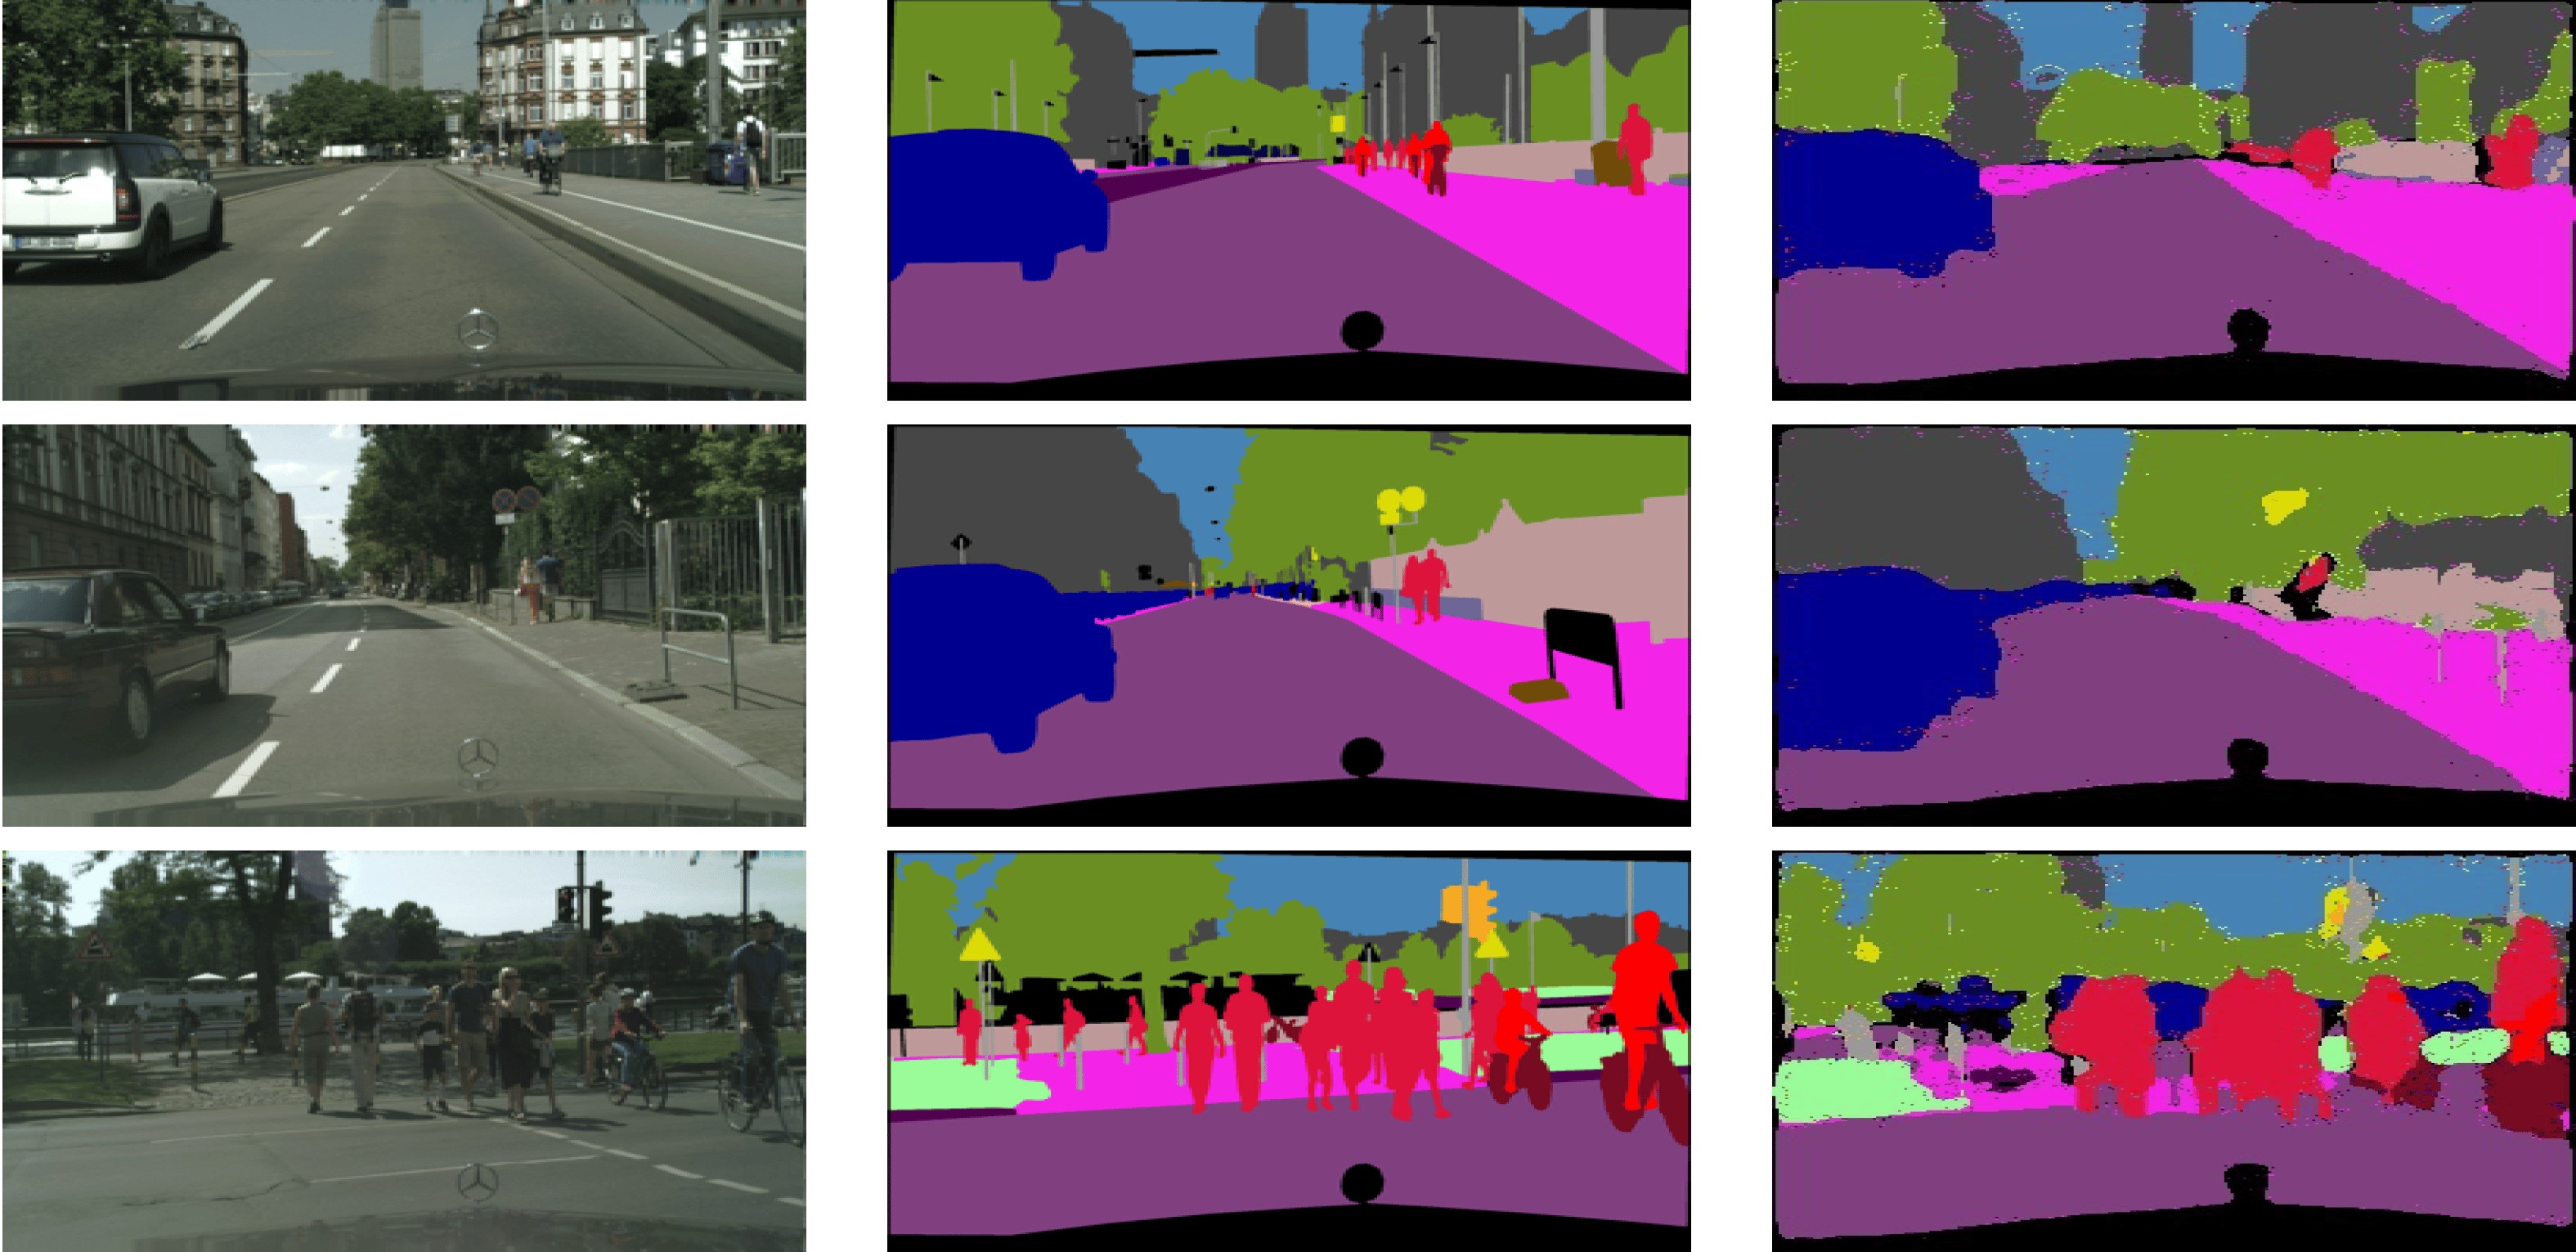
\includegraphics[width=1\textwidth]{bilder/autonomous_driving2.jpg}
    \captionsetup{font=small} % Hier die gewünschte Größe einstellen
    \caption[semantische Segmentierung im Bereich des autonomen Fahrens]{semantische Segmentierung im Bereich des autonomen Fahrens, Ursprungsbild (links), Ground Truth (mitte), Segmentierungsergebnis (rechts) \cite{madokoro2022semantic}}
    \label{fig:SS_auto}
\end{figure}

\section{Robotik in der Industrie}

Die semantische Segmentierung spielt eine wichtige Rolle in der
Industrierobotik, insbesondere wenn es darum geht, stark variierende Produkte
bezüglich ihres Formfaktors zu handhaben. Eine Herausforderung besteht darin,
die Produkte zu erkennen und zu klassifizieren. Dies ermöglicht es dem Roboter
zwischen unterschiedlichen Teilen zu unterscheiden und bauteilspezifisch zu
reagieren. So kann beispielsweise eine optimale Griffposition des Bauteils
ermittelt oder Objekten beim Anfahren gezielt ausgewichen werden. Eine
solche Problemstellung ist dabei in \ref{fig:SS_robotics} zu erkennen. Auch
eine Manipulation komplexer Objekte kann dadurch ermöglicht werden.
\cite{liu2020real}

\begin{figure}[h]
    \centering
    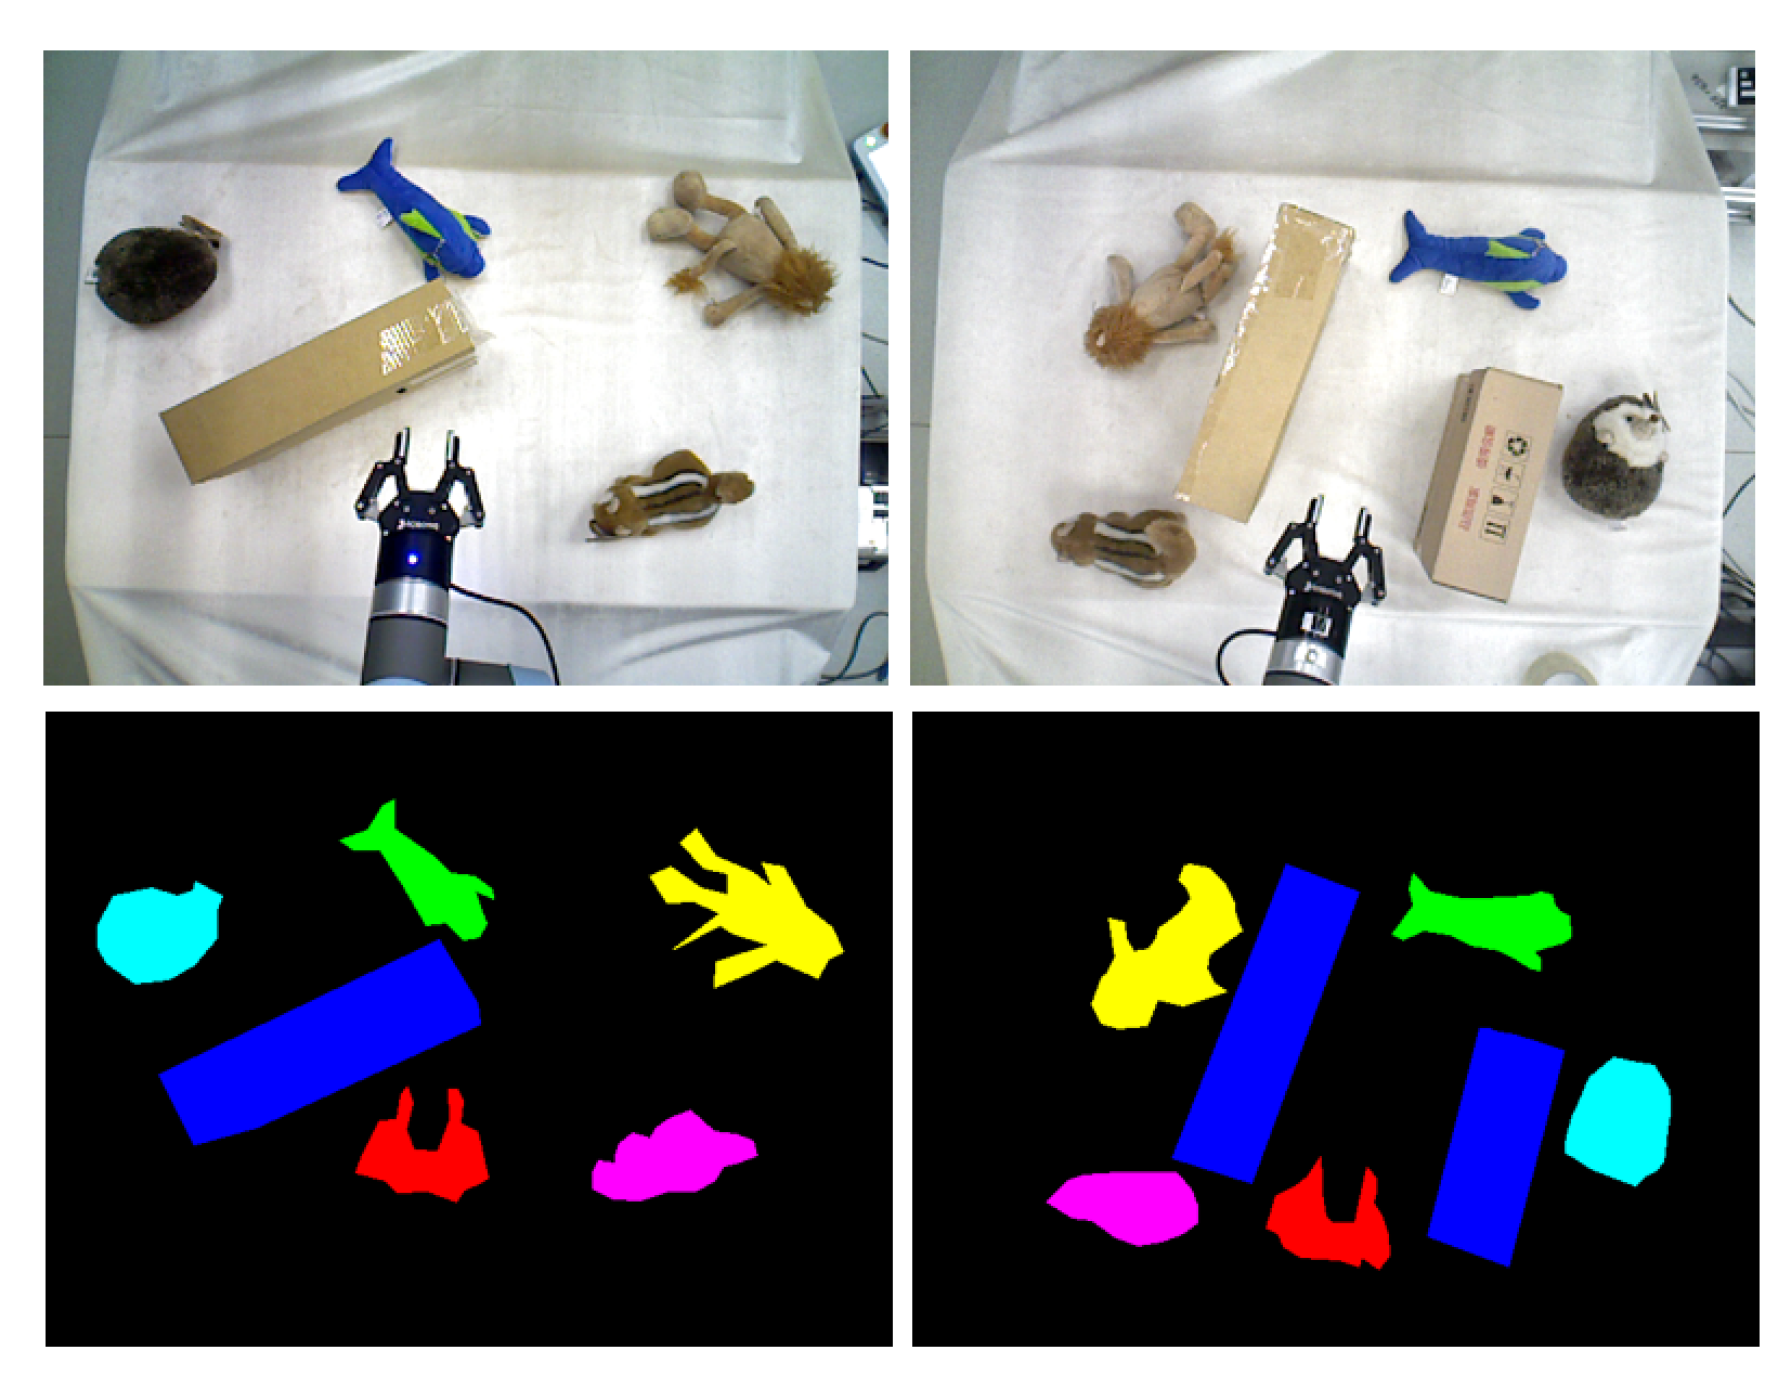
\includegraphics[width=1\textwidth]{bilder/semantic_segmentation_Robotics.png}
    \captionsetup{font=small} % Hier die gewünschte Größe einstellen

    \caption[semantische Segmentierung in der industrierobotik]{semantische Segmentierung in der Industrierobotik \cite{liu2020real}}
    \label{fig:SS_robotics}
\end{figure}

\section{Augmented Reality}
Einsatzgebiete der semantischen Segmentierung im Bereich von Augmented Reality
(AR) sind vielfältig. Diese kann beispielsweise in der industriellen Fertigung
eingesetzt werden, um komplexe Montage- und Wartungsprozesse zu unterstützen.
Durch semantische Segmentierung können AR-Systeme bereits platzierte Teile und
Komponenten identifizieren, Fehler erkennen und den Arbeitern visuelle
Montageanleitungen in Echtzeit bereitstellen. Dies erhöht die Effizienz,
Präzision und Sicherheit bei der Durchführung von Aufgaben. In der Architektur
und im Bauwesen ermöglicht die semantische Segmentierung in Kombination mit AR
eine Visualisierung von Gebäuden und Infrastrukturen. Architekten, Designer und
Ingenieure können virtuelle Modelle in die reale Umgebung einfügen, um Entwürfe
auf Kollisionen zu überprüfen. Die semantische Segmentierung ist dabei eine
entscheidende Komponente, um die Umgebung zu analysieren, zu verstehen und
interaktiv nutzbar zu machen. Dies ermöglicht es AR-Systemen, die Umgebung zu
analysieren und virtuelle Inhalte realitätsnah zu platzieren und mit diesen zu
interagieren. Abbildung \ref{fig:SS_medizin} zeigt dabei eine bestehende
Anwendung von AR im Bereich der Medizin. \cite{nee2012augmented,ko2020novel}

\section{Landwirtschaft}

Auch in der Landwirtschaft hat die semantische Segmentierung große Potenziale.
Durch die präzise Klassifizierung von verschiedenen Pflanzenarten und
Strukturen auf landwirtschaftlichen Flächen, können Landwirte wichtige
Informationen gewinnen, um ihre Produktivität und Effizienz zu steigern. Mit
Hilfe der semantischen Segmentierung können Unkraut und Nutzpflanzen
unterschieden werden, wie in Abbildung \ref{fig:SS_landwirtschaft} dargestellt
ist. Dies ermöglicht eine gezielte Anwendung von Düngemitteln und Pestiziden,
sowie einer effizienten Bewässerung. Darüber hinaus kann die semantische
Segmentierung auch bei der Erkennung von Schädlingen und Krankheiten helfen, um
rechtzeitig Gegenmaßnahmen zu ergreifen. Durch die genaue Analyse und
Segmentierung landwirtschaftlicher Flächen bietet die semantische Segmentierung
ein wertvolles Werkzeug, um die Landwirtschaft nachhaltiger, produktiver und
umweltfreundlicher zu gestalten. \cite{8460962}

\begin{figure}[h]
    \centering
    \includegraphics[width=1\textwidth]{bilder/semantic_segmentation_landwirtschaft.png}
    \captionsetup{font=small} % Hier die gewünschte Größe einstellen
    \caption[semantische Segmentierung in der Landwirtschaft]{semantische Segmentierung in der Landwirtschaft, Originalbild (links), Ground Truth (mitte), Segmentierungsergebnis (rechts) \cite{madokoro2022semantic}}
    \label{fig:SS_landwirtschaft}
\end{figure}

\section{Medizin}
Semantische Segmentierung spielt eine entscheidende Rolle im Bereich der
Medizintechnik und hat das Potenzial, unterstützend bei medizinische Diagnosen
und Behandlungen zu wirken. Durch die präzise Segmentierung von anatomischen
Strukturen und Geweberegionen in medizinischen Bildern wie CT-Scans
(Computertomographie-Scan) oder MRT-Aufnahmen
(Magnetresonanz-tomographie-Aufnahmen) können Ärzte einen besseren Einblick in
die Anatomie des Patienten erhalten. Beispielsweise können Organe für einen
besseren Überblick automatisch eingefärbt werden oder verdächtige Stellen in
der Aufnahme markiert werden. So kann der untersuchende Arzt beispielsweise
Verletzungen oder potenzielle Tumore gezielt betrachten. Diese detaillierte
Analyse ermöglicht eine präzisere Diagnosestellung und kann bei der Planung und
Durchführung von chirurgischen Eingriffen, sowie der Überwachung des
Fortschreitens von Krankheiten eingesetzt werden. Die semantische Segmentierung
erleichtert auch die Erstellung von 3D-Modellen anatomischer Strukturen, die
für die präoperative Planung und Simulation von komplexen Operationen verwendet
werden können. Dabei können beispielsweise markante Stellen einer CT-Aufnahme
bei einer endoskopischen Operation wieder erkannt werden und dem operierenden
Arzt unterstützend eingeblendet werden. Dies kann unter anderem auch mithilfe
von AR geschehen. Ein solcher Anwendungsfall ist in Abbildung
\ref{fig:SS_medizin} dargestellt. \cite{asgari2021deep,tanzi2021real}

\begin{figure}[H]
    \centering
    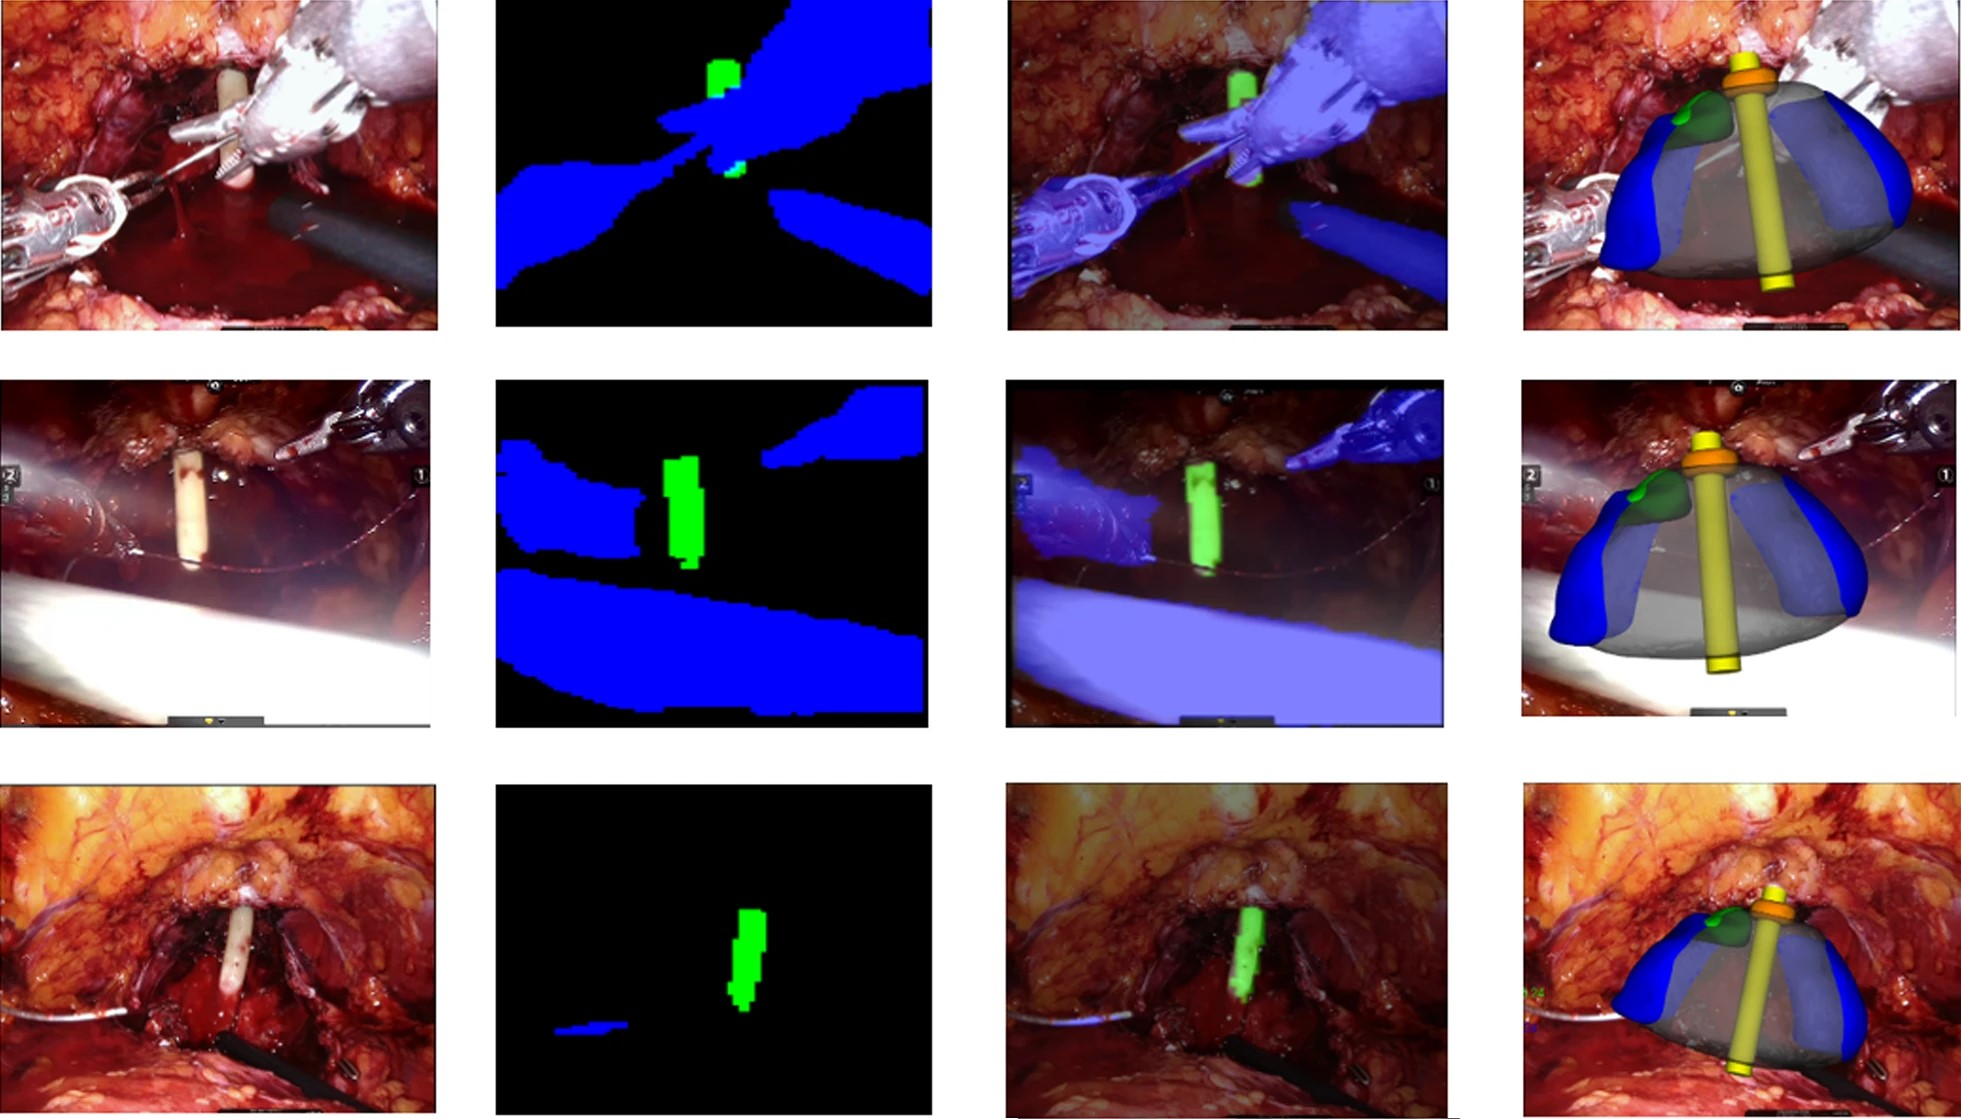
\includegraphics[width=1\textwidth]{bilder/medizin_AR.jpg}
    \captionsetup{font=small} % Hier die gewünschte Größe einstellen

    \caption[semantische Segmentierung im Bereich der Medizin, in Kombination mit Augmented Reality] {semantische Segmentierung im Bereich der Medizin, in Kombination mit Augmented Reality. Von links nach rechts: Originalbild, Segmentierungsergebnis, Overlay1, Overlay2.  \cite{tanzi2021real}}
    \label{fig:SS_medizin}
\end{figure}